\documentclass[10pt]{NSP1}

\usepackage{url,floatflt}
\usepackage{helvet,times}
\usepackage{psfig,graphics}
\usepackage{mathptmx,amsmath,amssymb,bm}
\usepackage{float}
\usepackage[bf,hypcap]{caption}
\usepackage[dvipsnames,table,xcdraw]{xcolor}
\usepackage{subfig}
\usepackage{hyperref}

\addtolength{\oddsidemargin}{.5in}
\addtolength{\evensidemargin}{-.5in}



\topmargin=0.00cm

\def\sm{\smallskip}
\def\no{\noindent}

% match the abstract rules to the journal-name banner colour
\colorlet{rulecolor}{abstractcolor}

\providecommand{\ul}[1]{#1}

\DeclareMathOperator{\sech}{sech}
\DeclareMathOperator{\csch}{csch}

\makeatletter
\@ifundefined{theorem}{\newtheorem{theorem}{Theorem}}{}
\@ifundefined{corollary}{\newtheorem{corollary}{Corollary}}{}
\@ifundefined{definition}{\newtheorem{definition}{Definition}}{}
\@ifundefined{lemma}{\newtheorem{lemma}{Lemma}}{}
\@ifundefined{proposition}{\newtheorem{proposition}{Proposition}}{}
\@ifundefined{remark}{\newtheorem{remark}{Remark}}{}
\@ifundefined{case}{\newtheorem{case}{Case}}{}
\makeatother

\def\firstpage{1}
\setcounter{page}{\firstpage}
\def\thevol{1}
\def\thenumber{1}
\def\theyear{2026}

\raggedbottom
\begin{document}

% body text enlarged ~5% (10pt -> 10.5pt) at the author's request
\makeatletter
\renewcommand\normalsize{\@setfontsize\normalsize{10.5}{12.6}}
\makeatother
\normalsize

\titlefigurecaption{{\large \bf \rm Progress in Fractional Differentiation
and Applications}\\ {\it\small An International Journal}}

\title{Analytical Dynamics of a Monkeypox Model Using Caputo-Fabrizio Fractional Derivative and Sumudu Transform Method}

\author{M. Ariyanatchi\hyperlink{author1}{$^{1}$}, Montasir Qasymeh\hyperlink{author2}{$^{2}$}, G.M. Vijayalakshmi\hyperlink{author3}{$^{3}$}, Paulraj Jayasimman\hyperlink{author4}{$^{4}$}, Roselyn Besi P.\hyperlink{author5}{$^{5}$}, Ali Akg\"ul\hyperlink{author6}{$^{6,7,*}$}, M. Abdel-Aty\hyperlink{author7}{$^{8,9,10}$} and M. Hafez\hyperlink{author8}{$^{11,12}$}}

\institute{Post Doctoral Fellow, Mathematics, AMET University, Chennai, India\and
Department of Electrical Engineering, Abu Dhabi University, Abu Dhabi, 59911, United Arab Emirates\and
Professor, Mathematics, Vel Tech Rangarajan Dr. Sagunthala R\&D Institute of Science and Technology, Chennai, India\and
Professor, Department of Mathematics, AMET University, Chennai, India\and
Coimbatore Institute of Technology, Coimbatore, India\and
Department of Electronics and Communication Engineering, Saveetha School of Engineering, SIMATS, Chennai, Tamilnadu, India\and
Siirt University, Art and Science Faculty, Department of Mathematics, 56100 Siirt, T\"urkiye\and
College of Engineering and Computing, Liwa University, Abu Dhabi, United Arab Emirates\and
Deanship of Graduate Studies and Research, Ahlia University, P.O. Box 10878, Manama, Bahrain\and
Mathematics Department, Faculty of Science, Sohag University, P.O. Box 82524, Sohag, Egypt\and
Faculty of Engineering and Quantity Surveying, INTI International University Colleges, Nilai, Malaysia\and
Faculty of Management, Shinawatra University, Pathum Thani, Thailand}

\titlerunning{Analytical dynamics of a Monkeypox Model...}

\authorrunning{M. Ariyanatchi et al.}

\mail{aliakgul@siirt.edu.tr, amisaty@gmail.com, mohdahmed.hafez@newinti.edu.my}

\received{---}
\revised{---}
\accepted{---}
\published{---}


\paperdoi{http://dx.doi.org/10.18576/pfda/120305}
\doi{http://dx.doi.org/10.18576/pfda/120305}
\abstracttext{This study presents a fractional-order mathematical model for the transmission dynamics of monkeypox, formulated using the Caputo-Fabrizio fractional derivative to better capture the memory and hereditary properties inherent in real-world biological systems. The model incorporates key epidemiological compartments to reflect the stages of monkeypox infection and transmission. To obtain analytical solutions, the Sumudu transform method is employed due to its efficiency in handling fractional differential equations. The existence and uniqueness of solutions are rigorously verified using fixed-point theory and the Picard--Lindelöf approach, ensuring mathematical consistency and reliability of the model. The proposed framework provides deeper insights into the progression of monkeypox and offers a robust analytical approach for studying disease dynamics under fractional-order settings. This work contributes significantly to understanding the impact of memory effects in disease modelling and can inform future control strategies for emerging infectious diseases like monkeypox.}

\keywords{Monkeypox, Fractional-Order Model, Caputo-Fabrizio Derivative, Sumudu Transform, Fixed-Point Theory, Picard-Lindel\"{o}f Approach, Disease Dynamics.}

\maketitle

\section{Introduction}

Mpox, formerly known as monkeypox, is a viral disease caused by the monkeypox virus (MPXV), part of the \emph{Orthopoxvirus} genus. There are two main clades: clade I (with subclades Ia and Ib) and clade II (with subclades IIa and IIb). The virus spreads through close contact with infected individuals, contaminated materials, or infected animals. It can also be transmitted during pregnancy or birth. Symptoms typically appear 1--21 days after exposure and include fever, rash, muscle aches, swollen lymph nodes, and low energy. The rash often progresses from flat sores to fluid-filled blisters that crust and fall off. While many recover within 2--4 weeks, severe cases can occur, especially in children, pregnant individuals, and people with weakened immune systems. Complications may include secondary infections, pneumonia, sepsis, encephalitis, or even death \cite{ref1,ref2,ref3}.

Diagnosis relies on PCR testing of lesions, while treatment focuses on symptom relief and supportive care, including hydration, nutrition, and management of pain and fever. Although there is no specific antiviral approved for mpox, some experimental antivirals are under evaluation. Vaccination, both pre- and post-exposure, is recommended for high-risk groups such as health workers, close contacts. During outbreaks, isolation, hygiene measures, and personal protective equipment (PPE) are essential to limit transmission \cite{ref4,ref5}. Mpox outbreaks have historically occurred in central and west Africa, with the first human case detected in 1970. However, the 2022--2023 global outbreak, driven by clade IIb, highlighted the disease's potential to spread rapidly across continents, reinforcing the importance of global surveillance, research, and public health preparedness \cite{ref6,ref7}.

Mathematical modelling is a valuable tool in understanding and managing the spread of monkeypox, especially due to its ability to simulate disease dynamics and assess intervention strategies. Because monkeypox was previously under-researched, early models helped identify critical factors like isolation and transmission pathways. A deterministic model presented in \cite{ref8} showed that isolating infected individuals could significantly reduce new infections. Similarly, the model developed in \cite{ref9} used nonlinear differential equations to examine how monkeypox spreads, revealing that a person's immune system influences recovery. More research works \cite{ref10,ref11,ref12,ref13} have expanded on this by studying different aspects of transmission and control strategies for infectious diseases. In \cite{ref14}, a model emphasized the role of non-pharmaceutical interventions in eliminating monkeypox outbreaks. Likewise, a simulation study in \cite{ref15} found that medical treatment can help remove the virus from both human and animal populations. Furthermore, recent models with environmental factors have been proposed in \cite{ref16,ref17} to better explain how monkeypox spread during the 2022 outbreak. These mathematical models play a key role in guiding public health policies and developing targeted prevention methods

Fractional calculus has become increasingly important in modelling real-world problems, particularly in disease dynamics, because of its unique ability to capture memory and hereditary effects---features often missing in classical models \cite{ref18,ref19,ref20,ref21,ref22}. In recent years, fractional-order models have been applied to infectious diseases like COVID-19 \cite{ref23,ref24,ref25,ref26,ref27}, providing more accurate results compared to traditional models. In \cite{ref28}, a stochastic fractional model was used to analyze cross-infection in monkeypox transmission, and \cite{ref29} introduced a fractal--fractional approach to study animal-to-human spread. Compared to standard derivatives, fractional derivatives allow better understanding of processes with long-term memory and time delays. Many researchers have used fractional models with Mittag--Leffler kernels and Caputo--Fabrizio operators for diseases such as dengue, Ebola, HIV/AIDS, and COVID-19 \cite{ref30,ref31,ref32,ref33,ref34,ref35,ref36,ref37,ref38,ref39}. In \cite{ref40}, Mittag--Leffler kernels helped model Ebola--malaria co-infections effectively, while \cite{ref41} used them to study HIV/AIDS, proving that infection rates could be reduced by adjusting fractional parameters. The Caputo--Fabrizio operator, known for its non-singular behaviour and exponential decay, has been preferred in works like \cite{ref40,ref41,ref42,ref43,ref44,ref45} for modelling typhoid, Alzheimer's, and other diseases. In \cite{ref46}, real-world data from Nigeria was used in a fractional model to evaluate control strategies for monkeypox, showing how mathematical analysis helps guide effective public health decisions. Similarly, \cite{ref47} confirmed that isolating infected people can control monkeypox transmission effectively. These studies highlight how fractional calculus significantly improves disease modelling and enhances predictive outcomes.

The Sumudu transform has emerged as an efficient tool for solving fractional-order differential equations due to its ability to preserve the original dimensionality of functions, ease of handling initial conditions, and compatibility with various fractional derivatives such as Caputo and Atangana-Baleanu. Compared to the Laplace transform, the Sumudu transform offers simpler inversion, operates in the real domain, and is often more suitable for physical systems with memory effects. In \cite{ref48}, the authors applied the Sumudu transform to a fractional COVID-19 model and demonstrated its effectiveness in capturing the epidemic dynamics with reduced computational complexity. Similarly, in {[}49{]}, a fractional model incorporating quarantine and isolation compartments was developed to assess containment strategies, highlighting the practical relevance of fractional derivatives in real-world epidemiological modelling.

The scope of this research lies in enhancing the analytical understanding of monkeypox dynamics by applying a fractional-order approach that accounts for the disease\textquotesingle s temporal memory characteristics. By structuring the model with relevant compartments and incorporating the Caputo-Fabrizio operator, the study addresses limitations of classical integer-order models in capturing delayed and hereditary effects in transmission. The use of the Sumudu transform offers a streamlined technique for solving the fractional system, allowing for more accessible and dimensionally consistent solutions. A key advantage of this study is its rigorous mathematical foundation, ensuring the existence and uniqueness of solutions through fixed-point techniques. Moreover, the model\textquotesingle s structure and methodology provide a flexible framework that can be extended to other infectious diseases, highlighting the potential of fractional modelling in supporting data-driven public health strategies.

In summary, this paper presents a comprehensive framework for modelling and controlling Dengue transmission using Caputo Fabrizio fractional derivatives and Sumudu transform techniques, offering significant improvements in disease management.

This paper is organized as follows: Section 2 presents the preliminary concepts and mathematical tools used in the study. Section 3 develops the fractional-order mathematical model for monkeypox transmission and introduces the key epidemiological compartments. Section 4 provides a qualitative analysis of the model, including existence and uniqueness of solutions. Section 5 focuses on the numerical analysis and simulation techniques. Section 6 discusses the results obtained from the simulations and interprets their epidemiological implications. Finally, Section 7 concludes the paper with a summary of findings and potential directions for future work.

\section{Preliminaries}

The Sumudu transform over the set of functions

\[
A = \left\{ F(t)|\exists M,\tau_{1},\tau_{2} > 0,\left| F(t) \right| < Me^{\frac{|t|}{\tau_{j}}},\ t \in ( - 1)^{j} \times \lbrack 0,\infty) \right\}
\]

Is defined as

\begin{equation}
G(u) = S\left\lbrack F(t) \right\rbrack = \int_{0}^{\infty}{}e^{- ut}\ F(t)dt
\end{equation}

The Sumudu transform of Caputo fractional derivative is explained below

\begin{equation}
ST\left\lbrack {0CD}_{t}^{\alpha}F(F,t):s \right\rbrack = s^{- \alpha}ST\left\{ F(F,t) \right\} - s^{- \alpha}\sum_{k = 0}^{m - 1}{}s^{k}F^{k}(F,0)
\end{equation}

The following definition of the Sumudu transform of Caputo-Fabrizio fractional differential coefficient of \(F(t)\) is based on the assumption that \(F(t)\) is a function whose Caputo-Fabrizio derivative occurs

\begin{equation}
ST\left( {0CfD}_{t}^{\alpha} \right)\left( F(t) \right) = M(\alpha)\left\lbrack \frac{ST\left( F(t) \right) - F(0)}{1 - \alpha + \alpha u} \right\rbrack
\end{equation}

\section{Model Formulation}

This study proposes a fractional-order differential equation model to describe the transmission dynamics of monkeypox involving interactions between two populations: humans and animals. Each population is subdivided into relevant epidemiological compartments to reflect the stages of infection and recovery.

Human Population Compartments:

The human population is divided into four compartments:

\begin{itemize}
\item
  \(S_{b}\): Susceptible humans
\item
  \(I_{b}\) : Infected humans
\item
  \(R_{b}\): Recovered humans
\item
  \(P_{b}\): Protected humans (e.g., through immunity or vaccination)
\end{itemize}

The total human population is denoted by \(N_{b} = S_{b} + I_{b}\) +\(R_{b} + P_{b}\). New individuals are recruited into the human population at a constant rate \(\pi_{b}\). Susceptible humans may become infected through contact with infected animals or other infected humans. The effective contact rate between susceptible humans and infected animals is represented by \(\beta_{b_{1}}\), and the contact rate between susceptible and infected humans is given by \(\beta_{b_{2}}\).

Infected humans recover at a rate \(\gamma_{b}\), while a proportion of recovered individuals move to the protected class at a rate \(\theta_{b}\). The model also accounts for the natural death rate \(\mu_{b}\) and disease-induced death rate \(d_{b}\) among the human population.

Animal Population Compartments:

The animal population is categorized into three compartments:

\begin{itemize}
\item
  \(S_{a}\): Susceptible animals
\item
  \(I_{a}\): Infected animals
\item
  \(R_{a}\): Recovered animals
\end{itemize}

The total animal population is \(N_{a} = S_{a}\)+\(I_{a} + R_{a}\). Animals are recruited at a rate \(\pi_{a}\). Susceptible animals can become infected through contact with infected animals at an effective contact rate \(\beta_{a}\). Infected animals recover at a rate \(\gamma_{a}\). The model includes both the natural death rate \(\mu_{a}\) and the disease-induced death rate \(d_{a}\) for animals.

Model Dynamics:

The transition of individuals between compartments is governed by a system of nonlinear differential equations that describe the rates of change in each compartment over time. The interaction terms, recruitment, recovery, protection, and mortality are all included to reflect realistic biological and epidemiological processes. This compartmental structure enables the model to capture the dynamics of monkeypox spread within and between human and animal populations.

\begin{equation}
\begin{aligned}
\frac{dS_{b}}{dt} &= \left( 1 - P_{b} \right)\pi_{b} - \frac{\left( \beta_{b_{1}}I_{a} + \beta_{b_{2}}I_{b} \right)S_{b}}{N_{b}} - \mu_{b}S_{b} \\
\frac{dI_{b}}{dt} &= \frac{\left( \beta_{b_{1}}I_{a} + \beta_{b_{2}}I_{b} \right)S_{b}}{N_{b}} - \left( \gamma_{b} + \mu_{b} + d_{b} \right)I_{b} \\
\frac{dR_{b}}{dt} &= \gamma_{b}I_{b} - \theta_{b}R_{b} - \mu_{b}R_{b} \\
\frac{dP_{b}}{dt} &= P_{b}\pi_{b} + \theta_{b}R_{b} - \mu_{b}P_{b} \\
\frac{dS_{a}}{dt} &= \pi_{a} - \frac{\beta_{a}S_{a}I_{a}}{N_{a}} - \mu_{a}S_{a} \\
\frac{dI_{a}}{dt} &= \frac{\beta_{a}S_{a}I_{a}}{N_{a}} - \left( \gamma_{a} + \mu_{a} + d_{a} \right)I_{a} \\
\frac{dR_{a}}{dt} &= \gamma_{a}I_{a} - \mu_{a}R_{a}
\end{aligned}
\end{equation}

The above differential equation (4) is converted using the Caputo-Fabrizio fractional derivative to incorporate memory effects and non-local behaviour in the system dynamics. This approach ensures a more accurate representation of real-world disease progression without singular kernel issues.

\begin{equation}
\begin{aligned}
{0CfD}_{t}^{\alpha}S_{b} &= \left( 1 - P_{b} \right)\pi_{b} - \frac{\left( \beta_{b_{1}}I_{a} + \beta_{b_{2}}I_{b} \right)S_{b}}{N_{b}} - \mu_{b}S_{b} \\
{0CfD}_{t}^{\alpha}I_{b} &= \frac{\left( \beta_{b_{1}}I_{a} + \beta_{b_{2}}I_{b} \right)S_{b}}{N_{b}} - \left( \gamma_{b} + \mu_{b} + d_{b} \right)I_{b} \\
{0CfD}_{t}^{\alpha}R_{b}\ &= \gamma_{b}I_{b} - \theta_{b}R_{b} - \mu_{b}R_{b} \\
{0CfD}_{t}^{\alpha}P_{b}\ &= P_{b}\pi_{b} + \theta_{b}R_{b} - \mu_{b}P_{b} \\
{0CfD}_{t}^{\alpha}S_{a}\ &= \pi_{a} - \frac{\beta_{a}S_{a}I_{a}}{N_{a}} - \mu_{a}S_{a} \\
{0CfD}_{t}^{\alpha}I_{a} &= \frac{\beta_{a}S_{a}I_{a}}{N_{a}} - \left( \gamma_{a} + \mu_{a} + d_{a} \right)I_{a} \\
{0CfD}_{t}^{\alpha}R_{a} &= \gamma_{a}I_{a} - \mu_{a}R_{a}
\end{aligned}
\end{equation}

These equations describe the dynamic evolution of the variables \(S_{b} \geq 0,I_{b} \geq 0,\ R_{b} \geq 0,\)

\(P_{b} \geq 0,S_{a} \geq 0,\ I_{a} \geq 0,\ R_{a} \geq 0\ \ \)over time within the framework of the proposed model. The Caputo Fabrizio fractional (\(CF\)), represented by \({0CfD}_{t}^{\alpha}\), where \(0\  < \eta < 1.\)

\begin{table}[htbp]
\begin{center}
\caption{Parameter values used in the proposed fuzzy fractional-order monkeypox transmission model.}
\label{tab1}
\begin{tabular}{|p{180pt}|p{158pt}|}
\hline
Parameter & Values \\
\hline
\(\pi_{b}\) & 0.0056 \\
\hline
\(\beta_{b_{1}}\) & 0.002 \\
\hline
\(\beta_{b_{2}}\) & 0.004 \\
\hline
\(\gamma_{b}\) & 0.094 \\
\hline
\(\theta_{b}\) & 0.025 \\
\hline
\(P_{b}\) & 0.02 \\
\hline
\(\mu_{b}\) & 0.01 \\
\hline
\(d_{b}\) & 0.005 \\
\hline
\(\pi_{a}\) & 0.001 \\
\hline
\(\beta_{a}\) & 0.04 \\
\hline
\(\gamma_{a}\) & 0.02 \\
\hline
\(\mu_{a}\) & 0.015 \\
\hline
\(d_{a}\) & 0.08 \\
\hline
\end{tabular}
\end{center}
\end{table}

\section{Qualitative Analysis}

\subsection{Existence of the Solutions of the Desired Model}

\textbf{Theorem 3.1}

Describe \(Q_{1},\ Q_{2},Q_{3},Q_{4},Q_{5},Q_{6},Q_{7}\) and explain how they relate to variables.

\textbf{Proof}

Transforming the aforementioned proposed system (5) into an integral equation system-

\begin{equation}
\begin{aligned}
S_{b}(t) - S_{b}(0) &= {0CFT}_{t}^{\alpha}\left\lbrack \left( 1 - P_{b} \right)\pi_{b} - \frac{\left( \beta_{b_{1}}I_{a} + \beta_{b_{2}}I_{b} \right)S_{b}}{N_{b}} - \mu_{b}S_{b} \right\rbrack \\
{I_{b}(t) - I_{b}(0) = 0CFT}_{t}^{\alpha}\left\lbrack \frac{\left( \beta_{b_{1}}I_{a} + \beta_{b_{2}}I_{b} \right)S_{b}}{N_{b}} - \left( \gamma_{b} + \mu_{b} + d_{b} \right)I_{b} \right\rbrack \\
R_{b}(t) - R_{b}(0) &= {0CFT}_{t}^{\alpha}\left\lbrack \gamma_{b}I_{b} - \theta_{b}R_{b} - \mu_{b}R_{b} \right\rbrack \\
P_{b}(t) - P_{b}(0) &= {0CFT}_{t}^{\alpha}\left\lbrack \pi_{b}P_{b} + \theta_{b}R_{b} - \mu_{b}P_{b} \right\rbrack \\
S_{a}(t) - S_{a}(0) &= {0CFT}_{t}^{\alpha}\left\lbrack \pi_{a} - \frac{\beta_{a}S_{a}I_{a}}{N_{a}} - \mu_{a}S_{a} \right\rbrack \\
I_{a}(t) - I_{a}(0) &= {0CFT}_{t}^{\alpha}\left\lbrack \frac{\beta_{a}S_{a}I_{a}}{N_{a}} - \left( \gamma_{a} + \mu_{a} + d_{a} \right)I_{a} \right\rbrack \\
R_{a}(t) - R_{a}(0) &= {0CFT}_{t}^{\alpha}\left\lbrack \gamma_{a}I_{a} - \mu_{a}R_{a} \right\rbrack
\end{aligned}
\end{equation}

Using Nieto's definition, we then arrive at,

\begin{equation}
\begin{aligned}
S_{b}(t) &= S_{b}(0) + \frac{2(1 - \alpha)}{(2 - \alpha)M(\alpha)}\left\lbrack \left( 1 - P_{b}(t) \right)\pi_{b} - \frac{\left( \beta_{b_{1}}I_{a}(t) + \beta_{b_{2}}I_{b}(t) \right)S_{b}(t)}{N_{b}(t)} - \mu_{b}S_{b}(t) \right\rbrack \\
&\quad + \frac{2\alpha}{(2 - \alpha)M(\alpha)}\int_{0}^{t}{}\left\lbrack \left( 1 - P_{b}(s) \right)\pi_{b} - \frac{\left( \beta_{b_{1}}I_{a}(s) + \beta_{b_{2}}I_{b}(s) \right)S_{b}(s)}{N_{b}(t)} - \mu_{b}S_{b}(s) \right\rbrack ds \\
I_{b}(t) &= I_{b}(0) + \frac{2(1 - \alpha)}{(2 - \alpha)M(\alpha)}\left\lbrack \frac{\left( \beta_{b_{1}}I_{a}(t) + \beta_{b_{2}}I_{b}(t) \right)S_{b}(t)}{N_{b}(t)} - \left( \gamma_{b} + \mu_{b} + d_{b} \right)I_{b}(t) \right\rbrack \\
&\quad + \frac{2\alpha}{(2 - \alpha)M(\alpha)}\int_{0}^{t}{}\left\lbrack \frac{\left( \beta_{b_{1}}I_{a}(s) + \beta_{b_{2}}I_{b}(s) \right)S_{b}(s)}{N_{b}(s)} - \left( \gamma_{b} + \mu_{b} + d_{b} \right)I_{b}(s) \right\rbrack ds \\
R_{b}(t) &= R_{b}(0) + \frac{2(1 - \alpha)}{(2 - \alpha)M(\alpha)}\left\lbrack \gamma_{b}I_{b}(t) - \theta_{b}R_{b}(t) - \mu_{b}R_{b}(t) \right\rbrack \\
&\quad + \frac{2\alpha}{(2 - \alpha)M(\alpha)}\int_{0}^{t}{}\left\lbrack \gamma_{b}I_{b}(s) - \theta_{b}R_{b}(s) - \mu_{b}R_{b}(s) \right\rbrack ds \\
P_{b}(t) &= P_{b}(0) + \frac{2(1 - \alpha)}{(2 - \alpha)M(\alpha)}\left\lbrack \pi_{b}P_{b}(t) + \theta_{b}R_{b}(t) - \mu_{b}P_{b}(t) \right\rbrack \\
&\quad + \frac{2\alpha}{(2 - \alpha)M(\alpha)}\int_{0}^{t}{}\left\lbrack \pi_{b}P_{b}(s) + \theta_{b}R_{b}(s) - \mu_{b}P_{b}(s) \right\rbrack ds \\
S_{a}(t) &= S_{a}(0) + \frac{2(1 - \alpha)}{(2 - \alpha)M(\alpha)}\left\lbrack \pi_{a} - \frac{\beta_{a}S_{a}(t)I_{a}(t)}{N_{a}(t)} - \mu_{a}S_{a}(t) \right\rbrack \\
&\quad + \frac{2\alpha}{(2 - \alpha)M(\alpha)}\int_{0}^{t}{}\left\lbrack \pi_{a} - \frac{\beta_{a}S_{a}(s)I_{a}(s)}{N_{a}(s)} - \mu_{a}S_{a}(s) \right\rbrack ds \\
I_{a}(t) &= I_{a}(0) + \frac{2(1 - \alpha)}{(2 - \alpha)M(\alpha)}\left\lbrack \frac{\beta_{a}S_{a}{(t)I}_{a}(t)}{N_{a}(t)} - \left( \gamma_{a} + \mu_{a} + d_{a} \right)I_{a}(t) \right\rbrack \\
&\quad + \frac{2\alpha}{(2 - \alpha)M(\alpha)}\int_{0}^{t}{}\left\lbrack \frac{\beta_{a}S_{a}{(s)I}_{a}(s)}{N_{a}(s)} - \left( \gamma_{a} + \mu_{a} + d_{a} \right)I_{a}(s) \right\rbrack ds \\
R_{a}(t) &= R_{a}(0) + \frac{2(1 - \alpha)}{(2 - \alpha)M(\alpha)}\left\lbrack \gamma_{a}I_{a}(t) - \mu_{a}R_{a}(t) \right\rbrack \\
&\quad + \frac{2\alpha}{(2 - \alpha)M(\alpha)}\int_{0}^{t}{}\left\lbrack \gamma_{a}I_{a}(s) - \mu_{a}R_{a}(s) \right\rbrack ds
\end{aligned}
\end{equation}

Let's now assume that the kernels are provided as

\begin{equation}
\begin{aligned}
Q_{1}\left( t,S_{b} \right) &= \left( 1 - P_{b}(t) \right)\pi_{b} - \frac{\left( \beta_{b_{1}}I_{a}(t) + \beta_{b_{2}}I_{b}(t) \right)S_{b}(t)}{N_{b}(t)} - \mu_{b}S_{b}(t) \\
Q_{2}\left( t,I_{b} \right) &= \frac{\left( \beta_{b_{1}}I_{a}(t) + \beta_{b_{2}}I_{b}(t) \right)S_{b}(t)}{N_{b}(t)} - \left( \gamma_{b} + \mu_{b} + d_{b} \right)I_{b}(t) \\
Q_{3}\left( t,R_{b} \right) &= \gamma_{b}I_{b}(t) - \theta_{b}R_{b}(t) - \mu_{b}R_{b}(t) \\
Q_{4}\left( t,P_{b} \right) &= \pi_{b}P_{b}(t) + \theta_{b}R_{b}(t) - \mu_{b}P_{b}(t) \\
Q_{5}\left( t,S_{a} \right) &= \pi_{a} - \frac{\beta_{a}S_{a}(t)I_{a}(t)}{N_{a}(t)} - \mu_{a}S_{a}(t) \\
Q_{6}\left( t,I_{a} \right) &= \frac{\beta_{a}S_{a}{(t)I}_{a}(t)}{N_{a}(t)} - \left( \gamma_{a} + \mu_{a} + d_{a} \right)I_{a}(t) \\
Q_{7}\left( t,R_{a} \right) &= \gamma_{a}I_{a}(t) - \mu_{a}R_{a}(t)
\end{aligned}
\end{equation}

\newpage
\textbf{Theorem 3.2}

Demonstrate that \(Q_{1},\ Q_{2},Q_{3},Q_{4},Q_{5},Q_{6}\) and\(\ Q_{7}\) fulfil the Lipschitz requirement.

\textbf{Proof}

We will first demonstrate this for \(Q_{1}\). Considering that \(S_{b}\) and \({S_{b}}_{1}\) are any two functions, we have

~


\[
\| Q_{1}\left( t,S_{b} \right) - Q_{1}\left( t,{S_{b}}_{1} \right)\| = \| - \frac{\left( \beta_{b_{1}}I_{a}(t) + \beta_{b_{2}}I_{b}(t) \right)}{N_{b}(t)}S_{b}(t) - \mu_{b}S_{b}(t) + \frac{\left( \beta_{b_{1}}I_{a}(t) + \beta_{b_{2}}I_{b}(t) \right)}{N_{b}(t)}{S_{b}}_{1}(t) + \mu_{b}{S_{b}}_{1}(t)\|
\]


~


\begin{quote}
\(\leq \| - \left( \frac{\left( \beta_{b_{1}}I_{a}(t) + \beta_{b_{2}}I_{b}(t) \right)}{N_{b}(t)} + \mu_{b} \right)\|\| S_{b}(t) - {S_{b}}_{1}(t)\|\)
\end{quote}


~


\[
\| Q_{1}\left( t,S_{b} \right) - Q_{1}\left( t,{S_{b}}_{1} \right)\| \leq H_{1}\| S_{b}(t) - {S_{b}}_{1}(t)\|
\]


~


Where \(\| - \left( \frac{\left( \beta_{b_{1}}I_{a}(t) + \beta_{b_{2}}I_{b}(t) \right)}{N_{b}(t)} + \mu_{b} \right)\| \leq H_{1} < 1\).


~


Similarly, we can have

{\small
\[
\begin{aligned}
&\| Q_{2}\left( t,I_{b} \right) - Q_{2}\left( t,{I_{b}}_{1} \right)\| \leq \|\frac{\left( \beta_{b_{1}}I_{a}(t) + \beta_{b_{2}}I_{b}(t) \right)S_{b}(t)}{N_{b}(t)} - \left( \gamma_{b} + \mu_{b} + d_{b} \right)I_{b}(t) \\
&\quad - \ \frac{\ \left( \ \beta_{b_{1}}I_{a}(t) + \beta_{b_{2}}I_{b}(t) \right)S_{b}(t)}{N_{b}(t)} + \left( \gamma_{b} + \mu_{b} + d_{b} \right){I_{b}}_{1}(t)\| \\
&\quad \leq \|\left( \gamma_{b} + \mu_{b} + d_{b} \right)\|\| I_{b}(t) - {I_{b}}_{1}(t)\| \\
&\| Q_{2}\left( t,I_{b} \right) - Q_{2}\left( t,{I_{b}}_{1} \right)\| \leq H_{2}\| I_{b}(t) - {I_{b}}_{1}(t)\|
\end{aligned}
\]
}


~


Where \(\|\left( \gamma_{b} + \mu_{b} + d_{b} \right)\| \leq H_{2} < 1\).

Now,

\[
\begin{aligned}
&\| Q_{3}\left( t,R_{b} \right) - Q_{3}\left( t,{R_{b}}_{1} \right)\| \leq \|\gamma_{b}I_{b}(t) - \theta_{b}R_{b}(t) - \mu_{b}R_{b}(t) - \gamma_{b}I_{b}(t) + \theta_{b}{R_{b}}_{1}(t) + \mu_{b}{R_{b}}_{1}(t)\| \\
&\quad \leq \|\left( \theta_{b} + \mu_{b} \right)\|\| R_{b}(t) - {R_{b}}_{1}(t)\| \\
&\| Q_{3}\left( t,R_{b} \right) - Q_{3}\left( t,{R_{b}}_{1} \right)\| \leq H_{3}\| R_{b}(t) - {R_{b}}_{1}(t)\|
\end{aligned}
\]

Where \(\|\left( \theta_{b} + \mu_{b} \right)\| \leq H_{3} < 1\).

and

\[
\| Q_{4}\left( t,P_{b} \right) - Q_{4}\left( t,{P_{b}}_{1} \right)\| \leq H_{4}\| P_{b}(t) - {P_{b}}_{1}(t)\|
\]

Where \(\|\left( \pi_{b} + \mu_{b} \right)\| \leq H_{4} < 1\)

\[
\| Q_{5}\left( t,S_{a} \right) - Q_{5}\left( t,{S_{a}}_{1} \right)\| \leq H_{5}\| S_{a}(t) - {S_{a}}_{1}(t)\|
\]

Where \(\|\left( \frac{\beta_{a}I_{a}(t)}{N_{a}(t)} + \mu_{a} \right)\| \leq H_{5} < 1\).

\[
\| Q_{6}\left( t,I_{a} \right) - Q_{6}\left( t,{I_{a}}_{1} \right)\| \leq H_{6}\| I_{a}(t) - {I_{a}}_{1}(t)\|
\]

Where \(\| - \left( \frac{\beta_{a}S_{a}}{N_{a}(t)} - \left( \gamma_{a} + \mu_{a} + d_{a} \right) \right)\| \leq H_{6} < 1\).

\(\| Q_{7}\left( t,R_{a} \right) - Q_{7}\left( t,{R_{a}}_{1} \right)\| \leq H_{7}\| R_{a}(t) - {R_{a}}_{1}(t)\|\) , Where \(\|\mu_{a}\| \leq H_{7} < 1.\)

Now consider the recurrence formula, we can acquire

\begin{equation}
\begin{aligned}
{S_{b}}_{r}(t) &= \frac{2(1 - \alpha)}{(2 - \alpha)M(\alpha)}Q_{1}\left( t,{S_{b}}_{r - 1} \right) + \frac{2\alpha}{(2 - \alpha)M(\alpha)}\int_{0}^{t}{}Q_{1}\left( s,{S_{b}}_{r - 1} \right)ds\ \\
{I_{b}}_{r}(t) &= \frac{2(1 - \alpha)}{(2 - \alpha)M(\alpha)}Q_{2}\left( t,{I_{b}}_{r - 1} \right) + \frac{2\alpha}{(2 - \alpha)M(\alpha)}\int_{0}^{t}{}Q_{2}\left( s,{I_{b}}_{r - 1} \right)ds\ \\
{R_{b}}_{r}(t) &= \frac{2(1 - \alpha)}{(2 - \alpha)M(\alpha)}Q_{3}\left( t,{R_{b}}_{r - 1} \right) + \frac{2\alpha}{(2 - \alpha)M(\alpha)}\int_{0}^{t}{}Q_{3}\left( s,{R_{b}}_{r - 1} \right)ds\ \\
{P_{b}}_{r}(t) &= \frac{2(1 - \alpha)}{(2 - \alpha)M(\alpha)}Q_{4}\left( t,{P_{b}}_{r - 1} \right) + \frac{2\alpha}{(2 - \alpha)M(\alpha)}\int_{0}^{t}{}Q_{4}\left( s,{P_{b}}_{r - 1} \right)ds\ \\
{S_{a}}_{r}(t) &= \frac{2(1 - \alpha)}{(2 - \alpha)M(\alpha)}Q_{5}\left( t,{S_{a}}_{r - 1} \right) + \frac{2\alpha}{(2 - \alpha)M(\alpha)}\int_{0}^{t}{}Q_{5}\left( s,{S_{a}}_{r - 1} \right)ds \\
{I_{a}}_{r}(t) &= \frac{2(1 - \alpha)}{(2 - \alpha)M(\alpha)}Q_{6}\left( t,{I_{a}}_{r - 1} \right) + \frac{2\alpha}{(2 - \alpha)M(\alpha)}\int_{0}^{t}{}Q_{6}\left( s,{I_{a}}_{r - 1} \right)ds \\
{R_{a}}_{r}(t) &= \frac{2(1 - \alpha)}{(2 - \alpha)M(\alpha)}Q_{7}\left( t,{R_{a}}_{r - 1} \right) + \frac{2\alpha}{(2 - \alpha)M(\alpha)}\int_{0}^{t}{}Q_{7}\left( s,{R_{a}}_{r - 1} \right)ds
\end{aligned}
\end{equation}

When a norm is used in the concept of majorizing, the distinction between sub-sequent terms that implies

\begin{equation}
\begin{aligned}
U_{r}(t) &= {S_{b}}_{r}(t) - {S_{b}}_{r - 1}(t) = \frac{2(1 - \alpha)}{(2 - \alpha)M(\alpha)}Q_{1}\left( t,{S_{b}}_{r - 1} \right) + \frac{2\alpha}{(2 - \alpha)M(\alpha)}\int_{0}^{t}{}Q_{1}\left( s,{S_{b}}_{r - 1} \right)ds \\
&\quad - \frac{2(1 - \alpha)}{(2 - \alpha)M(\alpha)}Q_{1}\left( t,{S_{b}}_{r - 2} \right) + \frac{2\alpha}{(2 - \alpha)M(\alpha)}\int_{0}^{t}{}Q_{1}\left( s,{S_{b}}_{r - 2} \right)ds
\end{aligned}
\end{equation}

\begin{equation}
\begin{aligned}
U_{r}(t) &= \frac{2(1 - \alpha)}{(2 - \alpha)M(\alpha)}Q_{1}\left( t,{S_{b}}_{r - 1} \right) - \frac{2(1 - \alpha)}{(2 - \alpha)M(\alpha)}Q_{1}\left( t,{S_{b}}_{r - 2} \right) \\
&\quad + \frac{2\alpha}{(2 - \alpha)M(\alpha)}\int_{0}^{t}{}\left\{ Q_{1}\left( s,{S_{b}}_{r - 1} \right) - Q_{1}\left( s,{S_{b}}_{r - 2} \right) \right\} ds
\end{aligned}
\end{equation}

Now

\[
\| U_{r}(t)\| = \|{S_{b}}_{r}(t) - {S_{b}}_{r - 1}(t)\|
\]

\begin{equation}
\begin{aligned}
&= \|\frac{2(1 - \alpha)}{(2 - \alpha)M(\alpha)}Q_{1}\left( t,{S_{b}}_{r - 1} \right) - \frac{2(1 - \alpha)}{(2 - \alpha)M(\alpha)}Q_{1}\left( t,{S_{b}}_{r - 2} \right) + \frac{2\alpha}{(2 - \alpha)M(\alpha)}\int_{0}^{t}{}\left\{ Q_{1}\left( s,{S_{b}}_{r - 1} \right) - Q_{1}\left( s,{S_{b}}_{r - 2} \right) \right\} ds\| \\
&\leq \frac{2(1 - \alpha)}{(2 - \alpha)M(\alpha)}\| Q_{1}\left( t,{S_{b}}_{r - 1} \right) - Q_{1}\left( t,{S_{b}}_{r - 2} \right)\| + \frac{2\alpha}{(2 - \alpha)M(\alpha)}\|\int_{0}^{t}{}\left\{ Q_{1}\left( s,{S_{b}}_{r - 1} \right) - Q_{1}\left( s,{S_{b}}_{r - 2} \right) \right\} ds\|
\end{aligned}
\end{equation}

But \(Q_{1}\) satisfies Lipchitz condition so,

\begin{equation}
\| U_{r}(t)\| \leq \frac{2(1 - \alpha)}{(2 - \alpha)M(\alpha)}H_{1}\|{S_{b}}_{r - 1} - {S_{b}}_{r - 2}\| + \frac{2\alpha}{(2 - \alpha)M(\alpha)} \times \int_{0}^{t}{}K_{1}\|{S_{b}}_{r - 1} - {S_{b}}_{r - 2}\| ds
\end{equation}

In the same way, we have

\begin{equation}
\| V_{r}(t)\| \leq \frac{2(1 - \alpha)}{(2 - \alpha)M(\alpha)}H_{2}\|{I_{b}}_{r - 1} - {I_{b}}_{r - 2}\| + \frac{2\alpha}{(2 - \alpha)M(\alpha)} \times \int_{0}^{t}{}K_{2}\|{I_{b}}_{r - 1} - {I_{b}}_{r - 2}\| ds
\end{equation}

\begin{equation}
\| W_{r}(t)\| \leq \frac{2(1 - \alpha)}{(2 - \alpha)M(\alpha)}H_{3}\|{R_{b}}_{r - 1} - {R_{b}}_{r - 2}\| + \frac{2\alpha}{(2 - \alpha)M(\alpha)} \times \int_{0}^{t}{}K_{3}\|{R_{b}}_{r - 1} - {R_{b}}_{r - 2}\| ds
\end{equation}

\begin{equation}
\| T_{r}(t)\| \leq \frac{2(1 - \alpha)}{(2 - \alpha)M(\alpha)}H_{4}\|{P_{b}}_{r - 1} - {P_{b}}_{r - 2}\| + \frac{2\alpha}{(2 - \alpha)M(\alpha)} \times \int_{0}^{t}{}K_{4}\|{P_{b}}_{r - 1} - {P_{b}}_{r - 2}\| ds
\end{equation}

\begin{equation}
\| X_{r}(t)\| \leq \frac{2(1 - \alpha)}{(2 - \alpha)M(\alpha)}H_{5}\|{S_{a}}_{r - 1} - {S_{a}}_{r - 2}\| + \frac{2\alpha}{(2 - \alpha)M(\alpha)} \times \int_{0}^{t}{}K_{5}\|{S_{a}}_{r - 1} - {S_{a}}_{r - 2}\| ds
\end{equation}

\begin{equation}
\| Y_{r}(t)\| \leq \frac{2(1 - \alpha)}{(2 - \alpha)M(\alpha)}H_{6}\|{S_{m}}_{r - 1} - {S_{m}}_{r - 2}\| + \frac{2\alpha}{(2 - \alpha)M(\alpha)} \times \int_{0}^{t}{}K_{6}\|{I_{a}}_{r - 1} - {I_{a}}_{r - 2}\| ds
\end{equation}

\begin{equation}
\| Z_{r}(t)\| \leq \frac{2(1 - \alpha)}{(2 - \alpha)M(\alpha)}H_{7}\|{R_{a}}_{r - 1} - {R_{a}}_{r - 2}\| + \frac{2\alpha}{(2 - \alpha)M(\alpha)} \times \int_{0}^{t}{}K_{7}\|{R_{a}}_{r - 1} - {R_{a}}_{r - 2}\| ds
\end{equation}

\textbf{Theorem 3.3}

\begin{quote}
The outcome of suggested fractional order system (5) exists under the recommended operator.
\end{quote}

\textbf{Proof}

Using a recursive approach in above equation (13) - (19) presents the set of equation as follows

{\small
\begin{equation}
\| U_{r}(t)\| \leq \| S_{h}(0)\| + \left\{ \left( \frac{2(1 - \alpha)H_{1}}{(2 - \alpha)M(\alpha)} \right)^{r} \right\} + \left\{ \left( \frac{2\alpha K_{1}t}{(2 - \alpha)M(\alpha)} \right)^{r} \right\}
\end{equation}
}

{\small
\begin{equation}
\| V_{r}(t)\| \leq \| E_{h}(0)\| + \left\{ \left( \frac{2(1 - \alpha)H_{2}}{(2 - \alpha)M(\alpha)} \right)^{r} \right\} + \left\{ \left( \frac{2\eta K_{2}t}{(2 - \alpha)M(\alpha)} \right)^{r} \right\}
\end{equation}
}

{\small
\begin{equation}
\| W_{r}(t)\| \leq \| T_{h}(0)\| + \left\{ \left( \frac{2(1 - \alpha)H_{3}}{(2 - \alpha)M(\alpha)} \right)^{r} \right\} + \left\{ \left( \frac{2\eta K_{3}t}{(2 - \alpha)M(\alpha)} \right)^{r} \right\}
\end{equation}
}

{\small
\begin{equation}
\| T_{r}(t)\| \leq \| P_{b}(0)\| + \left\{ \left( \frac{2(1 - \alpha)H_{4}}{(2 - \alpha)M(\alpha)} \right)^{r} \right\} + \left\{ \left( \frac{2\eta K_{4}t}{(2 - \alpha)M(\alpha)} \right)^{r} \right\}
\end{equation}
}

{\small
\begin{equation}
\| X_{r}(t)\| \leq \| R_{h}(0)\| + \left\{ \left( \frac{2(1 - \alpha)H_{5}}{(2 - \alpha)M(\alpha)} \right)^{r} \right\} + \left\{ \left( \frac{2\alpha K_{5}t}{(2 - \alpha)M(\alpha)} \right)^{r} \right\}
\end{equation}
}

{\small
\begin{equation}
\| Y_{r}(t)\| \leq \| S_{m}(0)\| + \left\{ \left( \frac{2(1 - \alpha)H_{6}}{(2 - \alpha)M(\alpha)} \right)^{r} \right\} + \left\{ \left( \frac{2\alpha K_{6}t}{(2 - \alpha)M(\alpha)} \right)^{r} \right\}
\end{equation}
}

{\small
\begin{equation}
\| Z_{r}(t)\| \leq \| T_{m}(0)\| + \left\{ \left( \frac{2(1 - \alpha)H_{7}}{(2 - \alpha)M(\alpha)} \right)^{r} \right\} + \left\{ \left( \frac{2\alpha K_{7}t}{(2 - \alpha)M(\alpha)} \right)^{r} \right\}
\end{equation}
}

Consequently, the presence of results, which are also continuous, are confirmed.

We now get

\begin{equation}
\begin{aligned}
S_{b}(t) &= {S_{b}}_{r}(t) - E_{1,r}(t),I_{b}(t) = {I_{b}}_{r}(t) - E_{2,r}(t),I_{b}(t) = {I_{b}}_{r}(t) - E_{3,r}(t), \\
P_{b}(t) &= {P_{b}}_{r}(t) - E_{4,r}(t),\ S_{a}(t) = {S_{a}}_{r}(t) - E_{5,r}(t),\ I_{a}(t) = {I_{a}}_{r}(t) - E_{6,r}(t), \\
R_{a}(t) &= {R_{a}}_{r}(t) - E_{7,r}(t).
\end{aligned}
\end{equation}

Where \(E_{1,r}(t),E_{2,r}(t),E_{3,r}(t),E_{4,r}(t),E_{5,r}(t),E_{6,r}(t)\) and \(E_{7,r}(t)\) represent the series solution\textquotesingle s remaining terms. Consequently

\[
S_{h}(t) - {S_{h}}_{r}(t) = \frac{2(1 - \alpha)}{(2 - \alpha)M(\alpha)}Q_{1}\left( t,S_{h} - E_{1,r}(t) \right) + \frac{2\alpha}{(2 - \alpha)M(\alpha)} \times \int_{0}^{t}{}Q_{1}\left( s,S_{h} - E_{1,r}(s) \right)ds,
\]

\[
E_{h}(t) - {E_{h}}_{r}(t) = \frac{2(1 - \alpha)}{(2 - \alpha)M(\alpha)}Q_{2}\left( t,E_{h} - E_{2,r}(t) \right) + \frac{2\alpha}{(2 - \alpha)M(\alpha)} \times \int_{0}^{t}{}Q_{2}\left( s,E_{h} - E_{2,r}(s) \right)ds,
\]

\[
\begin{aligned}
T_{h}(t) - {T_{h}}_{r}(t) &= \frac{2(1 - \alpha)}{(2 - \alpha)M(\alpha)}Q_{3}\left( t,T_{h} - E_{3,r}(t) \right) + \frac{2\alpha}{(2 - \alpha)M(\alpha)} \times \int_{0}^{t}{}Q_{3}\left( s,T_{h} - E_{3,r}(s) \right)ds, \\
H_{h}(t) - {H_{h}}_{r}(t) &= \frac{2(1 - \alpha)}{(2 - \alpha)M(\alpha)}Q_{4}\left( t,H_{h} - E_{4,r}(t) \right) + \frac{2\alpha}{(2 - \alpha)M(\alpha)} \times \int_{0}^{t}{}Q_{4}\left( s,H_{h} - E_{4,r}(s) \right)ds
\end{aligned}
\]

\[
R_{h}(t) - {R_{h}}_{r}(t) = \frac{2(1 - \alpha)}{(2 - \alpha)M(\alpha)}Q_{5}\left( t,R_{h} - E_{5,r}(t) \right) + \frac{2\alpha}{(2 - \alpha)M(\alpha)} \times \int_{0}^{t}{}Q_{5}\left( s,R_{h} - E_{5,r}(s) \right)ds,
\]

\begin{equation}
\begin{aligned}
S_{m}(t) - {S_{m}}_{r}(t) &= \frac{2(1 - \alpha)}{(2 - \alpha)M(\alpha)}Q_{6}\left( t,S_{m} - E_{6,r}(t) \right) + \frac{2\alpha}{(2 - \alpha)M(\alpha)} \times \int_{0}^{t}{}Q_{6}\left( s,S_{m} - E_{6,r}(s) \right)ds \\
T_{m}(t) - {T_{m}}_{r}(t) &= \frac{2(1 - \alpha)}{(2 - \alpha)M(\alpha)}Q_{7}\left( t,T_{m} - E_{7,r}(t) \right) \\
&\quad + \frac{2\alpha}{(2 - \alpha)M(\alpha)} \times \int_{0}^{t}{}Q_{7}\left( s,T_{m} - E_{7,r}(s) \right)ds
\end{aligned}
\end{equation}


~


By applying the Lipschitz axiom and using the terms on both sides, the above claim is established.


~


{\small
\[
\begin{aligned}
&\| S_{h}(t) - \frac{2(1 - \alpha)Q_{1}\left( t,S_{h} \right)}{(2 - \alpha)M(\alpha)} - S_{h}(0) - \frac{2\alpha}{(2 - \alpha)M(\alpha)}\int_{0}^{t}{}Q_{1}\left( s,S_{h} \right)ds\| \\
&\quad \leq \| E_{1,r}(t)\|\left\{ 1 + \left( \frac{2(1 - \alpha)H_{1}}{(2 - \alpha)M(\alpha)} + \frac{2\alpha K_{1}t}{(2 - \alpha)M(\alpha)} \right) \right\} \\
&\| E_{h}(t) - \frac{2(1 - \alpha)Q_{2}\left( t,E_{h} \right)}{(2 - \alpha)M(\alpha)} - E_{h}(0) - \frac{2\alpha}{(2 - \alpha)M(\alpha)}\int_{0}^{t}{}Q_{2}\left( s,E_{h} \right)ds\| \\
&\quad \leq \| E_{2,r}(t)\|\left\{ 1 + \left( \frac{2(1 - \alpha)H_{2}}{(2 - \alpha)M(\alpha)} + \frac{2\alpha K_{2}t}{(2 - \alpha)M(\alpha)} \right) \right\} \\
&\| T_{h}(t) - \frac{2(1 - \alpha)Q_{3}\left( t,T_{h} \right)}{(2 - \alpha)M(\alpha)} - T_{h}(0) - \frac{2\alpha}{(2 - \alpha)M(\alpha)}\int_{0}^{t}{}Q_{3}\left( s,T_{h} \right)ds\| \\
&\quad \leq \| E_{3,r}(t)\|\left\{ 1 + \left( \frac{2(1 - \alpha)H_{3}}{(2 - \alpha)M(\alpha)} + \frac{2\alpha K_{3}t}{(2 - \alpha)M(\alpha)} \right) \right\} \\
&\| H_{h}(t) - \frac{2(1 - \alpha)Q_{4}\left( t,H_{h} \right)}{(2 - \alpha)M(\alpha)} - H_{h}(0) - \frac{2\alpha}{(2 - \alpha)M(\alpha)}\int_{0}^{t}{}Q_{4}\left( s,H_{h} \right)ds\|
\end{aligned}
\]
}


~


\[
\leq \| E_{4,r}(t)\|\left\{ 1 + \left( \frac{2(1 - \alpha)H_{4}}{(2 - \alpha)M(\alpha)} + \frac{2\alpha K_{4}t}{(2 - \alpha)M(\alpha)} \right) \right\},
\]


~


\[
\| R_{h}(t) - \frac{2(1 - \alpha)Q_{5}\left( t,R_{h} \right)}{(2 - \alpha)M(\alpha)} - R_{h}(0) - \frac{2\alpha}{(2 - \alpha)M(\alpha)}\int_{0}^{t}{}Q_{5}\left( s,R_{h} \right)ds\|
\]


~


\[
\leq \| E_{5,r}(t)\|\left\{ 1 + \left( \frac{2(1 - \alpha)H_{5}}{(2 - \alpha)M(\alpha)} + \frac{2\alpha K_{5}t}{(2 - \alpha)M(\alpha)} \right) \right\},
\]


~


\[
\| S_{m}(t) - \frac{2(1 - \alpha)Q_{6}\left( t,S_{m} \right)}{(2 - \alpha)M(\alpha)} - S_{m}(0) - \frac{2\alpha}{(2 - \alpha)M(\alpha)}\int_{0}^{t}{}Q_{6}\left( s,S_{m} \right)ds\|
\]


~


\[
\leq \| E_{6,r}(t)\|\left\{ 1 + \left( \frac{2(1 - \alpha)H_{6}}{(2 - \alpha)M(\alpha)} + \frac{2\alpha K_{6}t}{(2 - \alpha)M(\alpha)} \right) \right\},
\]


~


\begin{equation}
\begin{aligned}
&\| T_{m}(t) - \frac{2(1 - \alpha)Q_{7}\left( t,T_{m} \right)}{(2 - \alpha)M(\alpha)} - T_{m}(0) - \frac{2\alpha}{(2 - \alpha)M(\alpha)}\int_{0}^{t}{}Q_{7}\left( s,T_{m} \right)ds\| \\
&\quad \leq \| E_{7,r}(t)\|\left\{ 1 + \left( \frac{2(1 - \alpha)H_{7}}{(2 - \alpha)M(\alpha)} + \frac{2\alpha K_{7}t}{(2 - \alpha)M(\alpha)} \right) \right\}
\end{aligned}
\end{equation}

When lim\(\ r \rightarrow \infty\) is used, it indicates that

\small

\begin{equation}
\begin{aligned}
{S_{b}}_{h}(t) &= S_{b}(0) + \frac{2(1 - \alpha)Q_{1}\left( t,S_{b} \right)}{(2 - \alpha)M(\alpha)} + \frac{2\alpha}{(2 - \alpha)M(\alpha)}\int_{0}^{t}{}Q_{1}\left( s,S_{b} \right)ds \\
I_{b}(t) &= I_{b}(0) + \frac{2(1 - \eta)Q_{2}\left( t,I_{b} \right)}{(2 - \alpha)M(\alpha)} + \frac{2\alpha}{(2 - \alpha)M(\alpha)}\int_{0}^{t}{}Q_{2}\left( s,I_{b} \right)ds \\
R_{b}(t) &= R_{b}(0) + \frac{2(1 - \eta)Q_{3}\left( t,R_{b} \right)}{(2 - \alpha)M(\alpha)} + \frac{2\alpha}{(2 - \alpha)M(\alpha)}\int_{0}^{t}{}Q_{3}\left( s,R_{b} \right)ds \\
P_{b}(t) &= P_{b}(0) + \frac{2(1 - \eta)Q_{4}\left( t,P_{b} \right)}{(2 - \alpha)M(\alpha)} + \frac{2\alpha}{(2 - \alpha)M(\alpha)}\int_{0}^{t}{}Q_{4}\left( s,P_{b} \right)ds \\
S_{a}(t) &= S_{a}(0) + \frac{2(1 - \alpha)Q_{5}\left( t,S_{a} \right)}{(2 - \alpha)M(\alpha)} + \frac{2\alpha}{(2 - \alpha)M(\alpha)}\int_{0}^{t}{}Q_{5}\left( s,S_{a} \right)ds \\
I_{a}(t) &= I_{a}(0) + \frac{2(1 - \alpha)Q_{6}\left( t,I_{a} \right)}{(2 - \alpha)M(\alpha)} + \frac{2\alpha}{(2 - \alpha)M(\alpha)}\int_{0}^{t}{}Q_{6}\left( s,I_{a} \right)ds \\
R_{a}(t) &= R_{a}(0) + \frac{2(1 - \alpha)Q_{7}\left( t,R_{a} \right)}{(2 - \alpha)M(\alpha)} + \frac{2\alpha}{(2 - \alpha)M(\alpha)}\int_{0}^{t}{}Q_{7}\left( s,R_{a} \right)ds
\end{aligned}
\end{equation}

\normalsize

It demonstrates the results, such as the above-mentioned solutions as provided by the proposed model\textquotesingle s Eqn. (5).


\subsection{Uniqueness of Result}


In the following section, we will attempt to establish that the outcomes that were mentioned in the section that came before this one are completely independent. We presume that more sets of results are available for the configuration specified in Eqn. (29).




\textbf{Theorem 3.4}

The suggested fractional order epidemiological model Eqn. (5) has a unique solution.



\textbf{Proof}

We assume that \(\left( {S_{b}}_{1},{I_{b}}_{1},{R_{b}}_{1},{P_{b}}_{1},{S_{a}}_{1},{I_{a}}_{1},{R_{a}}_{1} \right)\)is also the solutions of suggested fractional model (5), based on the foundation of contradiction. Therefore


\begin{equation}
\begin{aligned}
S_{b}(t) - {S_{b}}_{1}(t) &= \frac{2(1 - \alpha)}{(2 - \alpha)M(\alpha)}\left\lbrack Q_{1}\left( t,S_{b} \right) - Q_{1}\left( t,{S_{b}}_{1} \right) \right\rbrack \\
&\quad + \frac{2\alpha}{(2 - \alpha)M(\alpha)}\int_{0}^{t}{}\left\lbrack Q_{1}\left( s,S_{b} \right) - Q_{1}\left( s,{S_{b}}_{1} \right) \right\rbrack ds
\end{aligned}
\end{equation}


Using the norm on both sides, we obtain



\begin{equation}
\begin{aligned}
\| S_{b} - {S_{b}}_{1}\| &= \frac{2(1 - \alpha)}{(2 - \alpha)M(\alpha)}\left\lbrack \| Q_{1}\left( t,S_{b} \right) - Q_{1}\left( t,{S_{b}}_{1} \right)\| \right\rbrack \\
&\quad + \frac{2\alpha}{(2 - \alpha)M(\alpha)}\int_{0}^{t}{}\left\lbrack \| Q_{1}\left( s,S_{b} \right) - Q_{1}\left( s,{S_{b}}_{1} \right)\| \right\rbrack ds
\end{aligned}
\end{equation}


Lipchitz condition is used to get




\begin{equation}
\| S_{b} - {S_{b}}_{1}\| < \frac{2(1 - \alpha)H_{1}}{(2 - \alpha)M(\alpha)} + \left( \frac{2\alpha K_{1}t}{(2 - \alpha)M(\alpha)} \right)^{r}
\end{equation}


Which is true for all\(\ r,\ \)so \(S_{b} = {S_{b}}_{1}\),


Similarly,\(\ I_{b} = {I_{b}}_{1}\),\(R_{b} = {R_{b}}_{1},P_{b} = {P_{b}}_{1}\),\(S_{a} = {S_{a}}_{1}\),\(I_{a} = {I_{a}}_{1}\) and \(R_{a} = {R_{a}}_{1}\).



Hence, it claims uniqueness of the system.

\section{Results of the Model Using Sumudu Transform with Caputo-Fabrizio Derivative}

Using the Caputo Fabrizio approach defined by the Sumudu Transform we obtain the following:

\small

\begin{equation}
\begin{aligned}
M(\alpha)\frac{ST\left( S_{b}(t) \right) - S_{b}(0)}{1 - \alpha + \Delta\alpha} &= ST\left\lbrack \left( 1 - P_{b} \right)\pi_{b} - \frac{\left( \beta_{b_{1}}I_{a} + \beta_{b_{2}}I_{b} \right)S_{b}}{N_{b}} - \mu_{b}S_{b} \right\rbrack \\
M(\alpha)\frac{ST\left( I_{b}(t) \right) - I_{b}(0)}{1 - \alpha + \Delta\alpha} &= ST\left\lbrack \frac{\left( \beta_{b_{1}}I_{a} + \beta_{b_{2}}I_{b} \right)S_{b}}{N_{b}} - \left( \gamma_{b} + \mu_{b} + d_{b} \right)I_{b} \right\rbrack \\
M(\alpha)\frac{ST\left( R_{b}(t) \right) - R_{b}(0)}{1 - \alpha + \Delta\alpha} &= ST\left\lbrack \gamma_{b}I_{b} - \theta_{b}R_{b} - \mu_{b}R_{b} \right\rbrack \\
M(\alpha)\frac{ST\left( P_{b}(t) \right) - P_{b}(0)}{1 - \alpha + \Delta\alpha} &= ST\left\lbrack \pi_{b}P_{b} + \theta_{b}R_{b} - \mu_{b}P_{b} \right\rbrack \\
M(\alpha)\frac{ST\left( S_{a}(t) \right) - S_{a}(0)}{1 - \alpha + \Delta\alpha} &= ST\left\lbrack \pi_{a} - \frac{\beta_{a}S_{a}I_{a}}{N_{a}} - \mu_{a}S_{a} \right\rbrack \\
M(\alpha)\frac{ST\left( I_{a}(t) \right) - I_{a}(0)}{1 - \alpha + \Delta\alpha} &= ST\left\lbrack \frac{\beta_{a}S_{a}I_{a}}{N_{a}} - \left( \gamma_{a} + \mu_{a} + d_{a} \right)I_{a} \right\rbrack \\
M(\alpha)\frac{ST\left( R_{a}(t) \right) - R_{a}(0)}{1 - \alpha + \Delta\alpha} &= ST\left\lbrack \gamma_{a}I_{a} - \mu_{a}R_{a} \right\rbrack
\end{aligned}
\end{equation}



By rearranging

\begin{equation}
\begin{aligned}
ST\left( S_{b}(t) \right) &= S_{b}(0) + \frac{1 - \alpha + \Delta\alpha}{M(\alpha)}ST\left\lbrack \left( 1 - P_{b} \right)\pi_{b} - \frac{\left( \beta_{b_{1}}I_{a} + \beta_{b_{2}}I_{b} \right)S_{b}}{N_{b}} - \mu_{b}S_{b} \right\rbrack \\
ST\left( I_{b}(t) \right) &= I_{b}(0) + \frac{1 - \alpha + \Delta\alpha}{M(\alpha)}ST\left\lbrack \frac{\left( \beta_{b_{1}}I_{a} + \beta_{b_{2}}I_{b} \right)S_{b}}{N_{b}} - \left( \gamma_{b} + \mu_{b} + d_{b} \right)I_{b} \right\rbrack \\
ST\left( R_{b}(t) \right) &= R_{b}(0) + \frac{1 - \alpha + \Delta\alpha}{M(\alpha)}ST\left\lbrack \gamma_{b}I_{b} - \theta_{b}R_{b} - \mu_{b}R_{b} \right\rbrack \\
ST\left( P_{b}(t) \right) &= H_{h}(0) + \frac{1 - \alpha + \Delta\alpha}{M(\alpha)}ST\left\lbrack \pi_{b}P_{b} + \theta_{b}R_{b} - \mu_{b}P_{b} \right\rbrack \\
ST\left( S_{a}(t) \right) &= S_{a}(0) + \frac{1 - \alpha + \Delta\alpha}{M(\alpha)}ST\left\lbrack \pi_{a} - \frac{\beta_{a}S_{a}I_{a}}{N_{a}} - \mu_{a}S_{a} \right\rbrack \\
ST\left( I_{a}(t) \right) &= I_{a}(0) + \frac{1 - \alpha + \Delta\alpha}{M(\alpha)}ST\left\lbrack \frac{\beta_{a}S_{a}I_{a}}{N_{a}} - \left( \gamma_{a} + \mu_{a} + d_{a} \right)I_{a} \right\rbrack \\
ST\left( R_{a}(t) \right) &= R_{a}(0) + \frac{1 - \alpha + \Delta\alpha}{M(\alpha)}ST\left\lbrack \gamma_{a}I_{a} - \mu_{a}R_{a} \right\rbrack
\end{aligned}
\end{equation}



Using inverse Sumudu transform on system (35), we get



\begin{equation}
\begin{aligned}
S_{b}(t) &= S_{b}(0) + {ST}^{- 1}\left\lbrack \frac{1 - \alpha + \Delta\alpha}{M(\alpha)}ST\left\lbrack \left( 1 - P_{b} \right)\pi_{b} - \frac{\left( \beta_{b_{1}}I_{a} + \beta_{b_{2}}I_{b} \right)S_{b}}{N_{b}} - \mu_{b}S_{b} \right\rbrack \right\rbrack \\
I_{b}(t) &= I_{b}(0) + {ST}^{- 1}\left\lbrack \frac{1 - \alpha + \Delta\alpha}{M(\alpha)}ST\left\lbrack \frac{\left( \beta_{b_{1}}I_{a} + \beta_{b_{2}}I_{b} \right)S_{b}}{N_{b}} - \left( \gamma_{b} + \mu_{b} + d_{b} \right)I_{b} \right\rbrack \right\rbrack \\
R_{b}(t) &= R_{b}(0) + {ST}^{- 1}\left\lbrack \frac{1 - \alpha + \Delta\alpha}{M(\alpha)}ST\left\lbrack \gamma_{b}I_{b} - \theta_{b}R_{b} - \mu_{b}R_{b} \right\rbrack \right\rbrack \\
P_{b}(t) &= P_{b}(0) + {ST}^{- 1}\left\lbrack \frac{1 - \alpha + \Delta\alpha}{M(\alpha)}ST\left\lbrack \pi_{b}P_{b} + \theta_{b}R_{b} - \mu_{b}P_{b} \right\rbrack \right\rbrack \\
S_{a}(t) &= S_{a}(0) + {ST}^{- 1}\left\lbrack \frac{1 - \alpha + \Delta\alpha}{M(\alpha)}ST\left\lbrack \pi_{a} - \frac{\beta_{a}S_{a}I_{a}}{N_{a}} - \mu_{a}S_{a} \right\rbrack \right\rbrack \\
I_{a}(t) &= I_{a}(0) + {ST}^{- 1}\left\lbrack \frac{1 - \alpha + \Delta\alpha}{M(\alpha)}ST\left\lbrack \frac{\beta_{a}S_{a}I_{a}}{N_{a}} - \left( \gamma_{a} + \mu_{a} + d_{a} \right)I_{a} \right\rbrack \right\rbrack \\
R_{a}(t) &= R_{a}(0) + {ST}^{- 1}\left\lbrack \frac{1 - \alpha + \Delta\alpha}{M(\alpha)}ST\left\lbrack \gamma_{a}I_{a} - \mu_{a}R_{a} \right\rbrack \right\rbrack
\end{aligned}
\end{equation}



Given recursive technique is as follows



\begin{equation}
\begin{aligned}
S_{b_{n + 1}}(t) &= S_{b_{n}}(0) + {ST}^{- 1}\left\lbrack \frac{1 - \alpha + \Delta\alpha}{M(\alpha)}ST\left\lbrack \left( 1 - P_{b_{n}} \right)\pi_{b} - \frac{\left( \beta_{b_{1}}I_{a_{n}} + \beta_{b_{2}}I_{b_{n}} \right)S_{b_{n}}}{N_{b}} - \mu_{b}S_{b_{n}} \right\rbrack \right\rbrack \\
I_{b_{n + 1}}(t) &= I_{b_{n}}(0) + {ST}^{- 1}\left\lbrack \frac{1 - \alpha + \Delta\alpha}{M(\alpha)}ST\left\lbrack \frac{\left( \beta_{b_{1}}I_{a_{n}} + \beta_{b_{2}}I_{b_{n}} \right)S_{b_{n}}}{N_{b}} - \left( \gamma_{b} + \mu_{b} + d_{b} \right)I_{b_{n}} \right\rbrack \right\rbrack \\
R_{b_{n + 1}}(t) &= R_{b_{n}}(0) + {ST}^{- 1}\left\lbrack \frac{1 - \alpha + \Delta\alpha}{M(\alpha)}ST\left\lbrack \gamma_{b}I_{b_{n}} - \theta_{b}R_{b_{n}} - \mu_{b}R_{b_{n}} \right\rbrack \right\rbrack \\
P_{b_{n + 1}}(t) &= P_{b_{n}}(0) + {ST}^{- 1}\left\lbrack \frac{1 - \alpha + \Delta\alpha}{M(\alpha)}ST\left\lbrack \pi_{b}P_{b_{n}} + \theta_{b}R_{b_{n}} - \mu_{b}P_{b_{n}} \right\rbrack \right\rbrack \\
S_{a_{n + 1}}(t) &= S_{a_{n}}(0) + {ST}^{- 1}\left\lbrack \frac{1 - \alpha + \Delta\alpha}{M(\alpha)}ST\left\lbrack \pi_{a} - \frac{\beta_{a}S_{a_{n}}I_{a_{n}}}{N_{a}} - \mu_{a}S_{a_{n}} \right\rbrack \right\rbrack \\
I_{a_{n + 1}}(t) &= I_{a_{n}}(0) + {ST}^{- 1}\left\lbrack \frac{1 - \alpha + \Delta\alpha}{M(\alpha)}ST\left\lbrack \frac{\beta_{a}S_{a_{n}}I_{a_{n}}}{N_{a}} - \left( \gamma_{a} + \mu_{a} + d_{a} \right)I_{a_{n}} \right\rbrack \right\rbrack \\
R_{a_{n + 1}}(t) &= R_{a_{n}}(0) + {ST}^{- 1}\left\lbrack \frac{1 - \alpha + \Delta\alpha}{M(\alpha)}ST\left\lbrack \gamma_{a}I_{a_{n}} - \mu_{a}R_{a_{n}} \right\rbrack \right\rbrack
\end{aligned}
\end{equation}

\normalsize

and the solution is given



\begin{equation}
\begin{aligned}
S_{b}(t) &= S_{b_{n}}(t)\ ,I_{b}(t) = I_{b_{n}}(t)\ ,R_{b}(t) = R_{b_{n}}(t)\ , \\
P_{b}(t) &= P_{b_{n}}(t)\ ,S_{a}(t) = S_{a_{n}}(t)\ ,I_{a}(t) = I_{a_{n}}(t)\ , \\
R_{a}(t) &= R_{a_{n}}(t)\ .
\end{aligned}
\end{equation}




\section{Result and Discussion}

This section presents the numerical simulations of the proposed monkeypox transmission model using the Sumudu transform method at varying fractional orders. The analysis is performed to understand how changes in the fractional order affect the progression of disease within human and animal populations. The simulations are conducted using MATLAB, based on Equation (38), and employ parameter values provided in Table 1. The results are visualized through Figures 1 to 3.


~


Figure 1 illustrates the transmission dynamics of monkeypox within the human population for three different fractional orders: 0.6, 0.8, and 1.0. At a lower fractional order of 0.6, the susceptible population declines more sharply, indicating that the infection spreads rapidly through the population during the initial stages. This sharper decline is attributed to the stronger memory effect present in systems of lower fractional order, which accelerates the movement between compartments. In contrast, at higher fractional orders of 0.8 and 1.0, the decline of the susceptible population is more gradual, suggesting a slower transmission rate and delayed progression of the infection. The infected population, however, grows more prominently at higher fractional orders. This suggests that with a weaker memory effect, the infection persists for longer durations and reaches a higher peak, especially in the case of the classical model (fractional order 1.0). The recovered and protected compartments also demonstrate increased accumulation at higher fractional orders, indicating that more individuals eventually transition out of infection as the system evolves more slowly over time. In lower fractional-order cases, the transitions are more rapid but result in fewer individuals being retained in the recovered or protected states over the simulated period.


~


Figure 2 focuses on the animal population dynamics under the same fractional orders. The behaviour observed in animal hosts complements the findings in the human population. The susceptible animal population shows a slower decline as the fractional order increases, reflecting a more prolonged exposure period and delayed transmission. Meanwhile, the infected and recovered animal populations display more significant growth at higher fractional orders, which is consistent with the reduced pace of change inherent in such systems. The gradual progression and delayed peak in the infected compartment at higher orders again highlight how fractional calculus, particularly with larger $\alpha$ values, slows the system evolution, thereby extending the duration of disease presence within the population. These simulations confirm that fractional-order modelling provides valuable insight into the real-world dynamical behaviour of infectious diseases, especially when memory effects and complex transitions are involved.


~


Figure 3 depicts the dynamics of the full proposed monkeypox model, incorporating both human and animal populations, based on real data from reported monkeypox cases in India as cited in \cite{ref48} and detailed in Table 1. Unlike Figures 1 and 2, this simulation is conducted with the model calibrated to actual outbreak data, providing a realistic picture of disease transmission and recovery patterns. The trajectories of the different compartments validate the model's capability to capture real epidemic behaviour. The simulation results align well with observed data, demonstrating the model\textquotesingle s effectiveness in portraying disease spread, peak infection periods, and eventual recovery dynamics. The consistency between the model outcomes and empirical data underscores the potential of using fractional-order systems in combination with the Sumudu transform to realistically represent complex infectious disease processes, offering better flexibility and accuracy in capturing delayed responses and memory-dependent phenomena.


~


In conclusion, the simulation outcomes underscore the significance of fractional-order parameters in shaping the transmission dynamics of monkeypox. Lower fractional orders accelerate transitions and reduce disease persistence, while higher orders induce slower, more sustained outbreaks. The Sumudu transform method proves effective in resolving the model equations, enabling clearer visualization and interpretation of complex system behavior under varying fractional dynamics.


\setlength{\floatsep}{0pt}     
\setlength{\textfloatsep}{0pt}  
\setlength{\intextsep}{0pt} 


\begin{figure}[H]
\centering
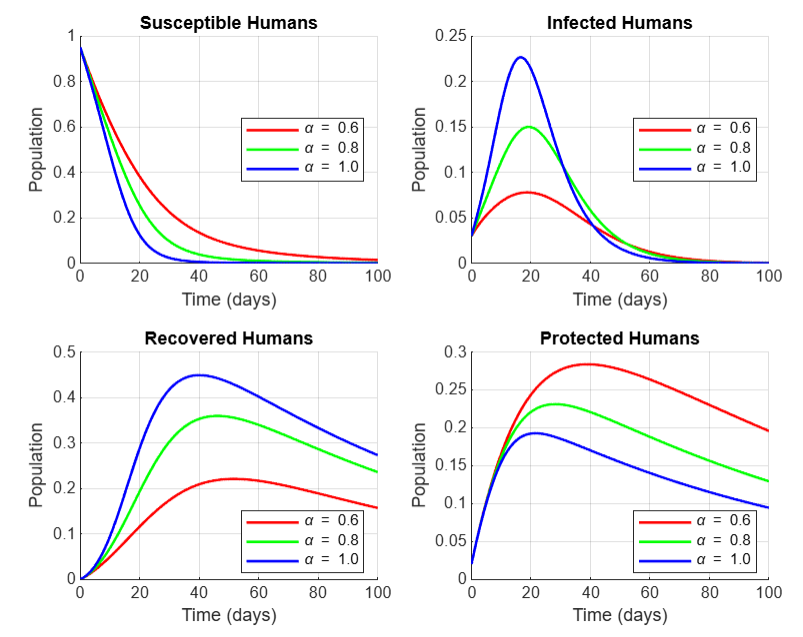
\includegraphics[width=5.5in, height=12cm]{media/fig1.png}
\caption{Transmission dynamics of monkeypox in the human population at different fractional orders (0.6, 0.8, and 1.0) using the Sumudu transform.}
\label{fig1}
\end{figure}

\begin{figure}[H]
\centering
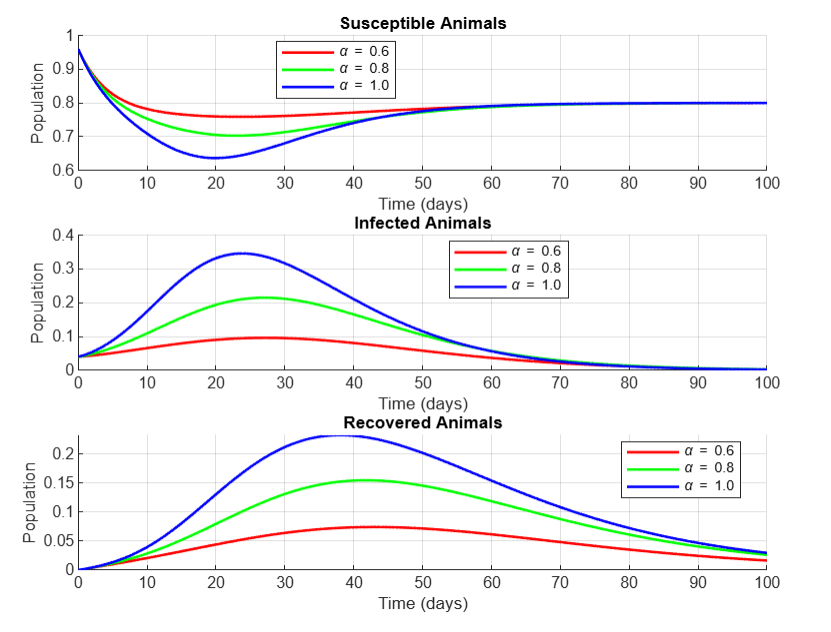
\includegraphics[width=5.5in, height=14cm]{media/fig2.png}
\caption{Animal population dynamics under different fractional orders (0.6, 0.8, and 1.0), showing variations in susceptible, infected, and recovered compartments.}
\label{fig2}
\end{figure}

\begin{figure}[H]
\centering
\subfloat{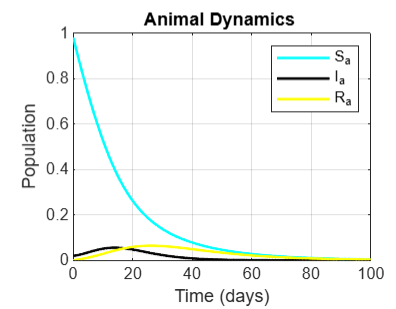
\includegraphics[width=2.70in,keepaspectratio]{media/fig3.1.png}}
\subfloat{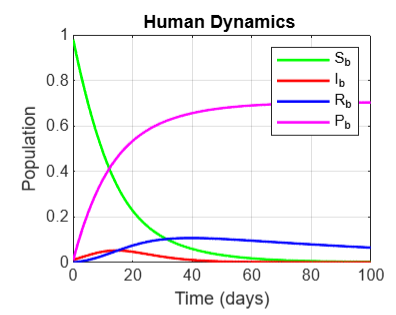
\includegraphics[width=2.70in,keepaspectratio]{media/fig3.2.png}}
\caption{Simulation of the proposed monkeypox model using real data, illustrating the disease progression across human and animal populations.}
\label{fig3}
\end{figure}

\section{Conclusion}

In this research, a novel fractional-order monkeypox transmission model has been developed using the Caputo-Fabrizio fractional derivative to effectively capture the memory and hereditary characteristics inherent in biological systems. By incorporating key epidemiological compartments, the model realistically reflects the stages of monkeypox infection and transmission. The Sumudu transform method was employed to derive analytical solutions, demonstrating its efficiency in handling fractional differential equations. To ensure the reliability of the results, the existence and uniqueness of solutions were established using fixed-point theory and the Picard--Lindelöf approach. This study offers several advantages, including the ability to model nonlocal and memory-dependent dynamics, a simplified analytical procedure through the Sumudu transform, and a mathematically rigorous framework that enhances the understanding of disease progression. The proposed model not only provides deeper insights into the complex behaviour of monkeypox spread but also serves as a valuable tool for informing public health strategies. Future research may focus on incorporating optimal control techniques to evaluate the effectiveness of intervention measures such as vaccination and public awareness campaigns, integrating real epidemiological data for validation, and extending the model to include spatial dynamics and stochastic influences for a more comprehensive representation of monkeypox outbreaks.

\textbf{Declaration of competing interest}

The authors declare there is no competing interest.

\textbf{Acknowledgement}

All authors have read and approved the article.

\textbf{Author's credit}

M.R have overall writing, M.A have conceptualised, J.P have supervised, G.M.V have validated and P.R.B have done visualisation.

\textbf{Funding}

No funding received.

\begin{thebibliography}{99}
\bibitem{aty1} Abdel-Aty, M., Abdel-Khalek, S., Obada, A.-S.F.
Pancharatnam phase of two-mode optical fields with Kerr nonlinearity, Optical Review, 2000, 7(6), pp. 499--504 DOI: \url{https://doi.org/10.1007/s10043-000-0499-6}

\bibitem{aty2} Rehman, H.U., Said, G.S., Amer, A., Elazab, N.S., Osman, M.S.
Unraveling the (4+1)-dimensional Davey-Stewartson-Kadomtsev-Petviashvili equation: Exploring soliton solutions via multiple techniques, Alexandria Engineering Journal, 2024, 90, pp. 17--23 DOI: \url{https://doi.org/10.1016/j.aej.2024.01.058}

\bibitem{aty3} Abdel-aty, M.
Quantum field entropy and entanglement of a three-level atom two-mode system with an arbitrary nonlinear medium, Journal of Modern Optics, 2003, 50(2), pp. 161--177 DOI: \url{https://doi.org/10.1080/09500340308235167}

\bibitem{aty4} El-Shahat, T.M., Abdel-Khalek, S., Abdel-Aty, M., Obada, A.-S.F.
Aspects on entropy squeezing of a two-level atom in a squeezed vacuum, Chaos Solitons and Fractals, 2003, 18(2), pp. 289--298 DOI: \url{https://doi.org/10.1016/S0960-0779(02)00652-5}

\bibitem{aty5} Obada, A.-S.F., Abdel-Aty, M.
Influence of the stark shift and kerr-like medium on the evolution of field entropy and entanglement in two-photon processes, Acta Physica Polonica B, 2000, 31(3), pp. 589--599 \url{https://www.actaphys.uj.edu.pl/R/31/3/589}

\bibitem{aty6} Abdel-Aty, M., Abdalla, M.S., Obada, A.-S.F.
Entropy and phase properties of isotropic coupled oscillators interacting with a single atom: one- and two-photon processes, Journal of Optics B Quantum and Semiclassical Optics, 2002, 4(3), pp. S133--S141 DOI: \url{https://doi.org/10.1088/1464-4266/4/3/367}

\bibitem{aty7} Zhang, J.-S., Chen, A.-X., Abdel-Aty, M.
Two atoms in dissipative cavities in dispersive limit: Entanglement sudden death and long-lived entanglement, Journal of Physics B Atomic Molecular and Optical Physics, 2010, 43(2), 025501 DOI: \url{https://doi.org/10.1088/0953-4075/43/2/025501}

\bibitem{aty8} Sebawe Abdalla, M., Hassan, S.S., Abdel-Aty, M.
Entropic uncertainty in the Jaynes-Cummings model in presence of a second harmonic generation, Optics Communications, 2005, 244(1-6), pp. 431--443 DOI: \url{https://doi.org/10.1016/j.optcom.2004.09.051}

\bibitem{aty9} Abdel-Aty, M.
An investigation of entanglement and quasiprobability distribution in a generalized Jaynes-Cummings model, Journal of Mathematical Physics, 2003, 44(4), pp. 1457--1471 DOI: \url{https://doi.org/10.1063/1.1559643}

\bibitem{aty10} Abdel-Aty, M., Sebawe Abdalla, M., Obada, A.-S.F.
Entropy squeezing of a two-mode multiphoton Jaynes-Cummings model in the presence of a nonlinear medium, Journal of Optics B Quantum and Semiclassical Optics, 2002, 4(2), pp. 134--142 DOI: \url{https://doi.org/10.1088/1464-4266/4/2/309}

\bibitem{ref1}
Sklenovská, N., \& Van Ranst, M. (2018). \emph{Emergence of monkeypox as the most important orthopoxvirus infection in humans}. Frontiers in Public Health, 6, 241. DOI: \url{https://doi.org/10.3389/fpubh.2018.00241}

\bibitem{ref2}
Centers for Disease Control and Prevention, National Center for Emerging and Zoonotic Infectious Diseases (NCEZID), Division of High-Consequence Pathogens and Pathology (DHCPP), Monkeypox (2021, accessed 11, Nov 2021).~\url{https://cdc.gov/poxvirus/monkeypox/index.html}

\bibitem{ref3}
Bunge, E. M., Hoet, B., Chen, L., Lienert, F., Weidenthaler, H., Baer, L. R., \& Steffen, R. (2022). \emph{The changing epidemiology of human monkeypox---A potential threat? A systematic review}. PLoS Neglected Tropical Diseases, 16(2), e0010141. DOI: \url{https://doi.org/10.1371/journal.pntd.0010141}

\bibitem{ref4}
Yinka-Ogunleye, A., Aruna, O., Dalhat, M., et al. (2018). \emph{Outbreak of human monkeypox in Nigeria in 2017--18: A clinical and epidemiological report}. The Lancet Infectious Diseases, 19(8), 872--879. DOI: \url{https://doi.org/10.1016/S1473-3099(19)30281-6}

\bibitem{ref5}
Thornhill, J. P., Barkati, S., Walmsley, S., et al. (2022). \emph{Monkeypox virus infection in humans across 16 countries --- April--June 2022}. New England Journal of Medicine, 387(8), 679--691. DOI: \url{https://doi.org/10.1056/NEJMoa2207323}

\bibitem{ref6}
Reynolds, M. G., Damon, I. K., \& McCollum, A. M. (2019). \emph{Vaccines and immunotherapeutics for monkeypox: A review of the current pipeline}. Vaccine, 37(43), 5995--6000. DOI: \url{https://doi.org/10.1016/j.vaccine.2019.08.016}

\bibitem{ref7}
Rao, A. K., Petersen, B. W., Whitehill, F., et al. (2022). \emph{Use of JYNNEOS (smallpox and monkeypox vaccine, live, nonreplicating) for preexposure vaccination of persons at risk for occupational exposure to orthopoxviruses: Recommendations of the Advisory Committee on Immunization Practices --- United States, 2022}. MMWR Morb Mortal Wkly Rep, 71(22), 734--742. DOI: \url{https://doi.org/10.15585/mmwr.mm7122e1}

\bibitem{ref8}
Peter, O. J., Kumar, S., Kumari, N., Oguntolu, F. A., Oshinubi, K., \& Musa, R. (2022). Transmission dynamics of Monkeypox virus: a mathematical modelling approach.~\emph{Modeling Earth Systems and Environment}, 8, 3423--3434. DOI: \url{https://doi.org/10.1007/s40808-021-01309-6}

\bibitem{ref9}
Ngungu, M., Addai, E., Adeniji, A., Adam, U. M., \& Oshinubi, K. (2023). Mathematical epidemiological modeling and analysis of monkeypox dynamism with non-pharmaceutical intervention using real data from United Kingdom.~\emph{Frontiers in Public Health},~\emph{11}, 1101436. DOI: \url{https://doi.org/10.3389/fpubh.2023.1101436}

\bibitem{ref10}
Baba, B. A., \& Bilgehan, B. (2021). Optimal control of a fractional order model for the COVID--19 pandemic.~\emph{Chaos, Solitons \& Fractals},~\emph{144}, 110678. DOI: \url{https://doi.org/10.1016/j.chaos.2021.110678}

\bibitem{ref11}
Ameen, I., Baleanu, D., \& Ali, H. M. (2020). An efficient algorithm for solving the fractional optimal control of SIRV epidemic model with a combination of vaccination and treatment.~\emph{Chaos, Solitons \& Fractals},~\emph{137}, 109892. DOI: \url{https://doi.org/10.1016/j.chaos.2020.109892}

\bibitem{ref12}
Abioye, A. I., Peter, O. J., Ogunseye, H. A., Oguntolu, F. A., Oshinubi, K., Ibrahim, A. A., \& Khan, I. (2021). Mathematical model of COVID-19 in Nigeria with optimal control.~\emph{Results in Physics},~\emph{28}, 104598. DOI: \url{https://doi.org/10.1016/j.rinp.2021.104598}

\bibitem{ref13}
Kumar, S., Chauhan, R. P., Momani, S., \& Hadid, S. (2024). Numerical investigations on COVID‐19 model through singular and non‐singular fractional operators.~\emph{Numerical Methods for Partial Differential Equations},~\emph{40}(1), e22707. DOI: \url{https://doi.org/10.1002/num.22707}

\bibitem{ref14}
Bankuru, S. V., Kossol, S., Hou, W., Mahmoudi, P., Rychtář, J., \& Taylor, D. (2020). A game-theoretic model of Monkeypox to assess vaccination strategies.~\emph{PeerJ},~\emph{8}, e9272. DOI: \url{https://doi.org/10.7717/peerj.9272}

\bibitem{ref15}
Usman, S., \& Adamu, I. I. (2017). Modeling the transmission dynamics of the monkeypox virus infection with treatment and vaccination interventions.~\emph{Journal of Applied Mathematics and Physics},~\emph{5}(12), 2335. DOI: \url{https://doi.org/10.4236/jamp.2017.512191}

\bibitem{ref16}
Alshehri, A., \& Ullah, S. (2023). Optimal control analysis of Monkeypox disease with the impact of environmental transmission.~\emph{Aims Math},~\emph{8}(7), 16926-16960. DOI: \url{https://doi.org/10.3934/math.2023865}

\bibitem{ref17}
Allehiany, F. M., DarAssi, M. H., Ahmad, I., Khan, M. A., \& Tag-Eldin, E. M. (2023). Mathematical modeling and backward bifurcation in monkeypox disease under real observed data.~\emph{Results in Physics},~\emph{50}, 106557. DOI: \url{https://doi.org/10.1016/j.rinp.2023.106557}

\bibitem{ref18}
Rihan, F. A., Baleanu, D., Lakshmanan, S., \& Rakkiyappan, R. (2014). On fractional SIRC model with salmonella bacterial infection. In~\emph{Abstract and Applied Analysis}~(Vol. 2014, No. 1, p. 136263). Hindawi Publishing Corporation. DOI: \url{https://doi.org/10.1155/2014/136263}

\bibitem{ref19}
Baba, I. A., \& Nasidi, B. A. (2021). Fractional order epidemic model for the dynamics of novel COVID-19.~\emph{Alexandria Engineering Journal},~\emph{60}(1), 537-548. DOI: \url{https://doi.org/10.1016/j.aej.2020.09.028}

\bibitem{ref20}
Rihan, F. A. (2013). Numerical modeling of fractional‐order biological systems. In~\emph{Abstract and applied analysis}~(Vol. 2013, No. 1, p. 816803). Hindawi Publishing Corporation. DOI: \url{https://doi.org/10.1155/2013/816803}

\bibitem{ref21}
Ali, A., Ullah, S., \& Khan, M. A. (2022). The impact of vaccination on the modeling of COVID-19 dynamics: a fractional order model.~\emph{Nonlinear Dynamics},~\emph{110}(4), 3921-3940. DOI: \url{https://doi.org/10.1007/s11071-022-07797-1}

\bibitem{ref22}
Saeedian, M., Khalighi, M., Azimi-Tafreshi, N., Jafari, G. R., \& Ausloos, M. (2017). Memory effects on epidemic evolution: The susceptible-infected-recovered epidemic model.~\emph{Physical Review E},~\emph{95}(2), 022409. DOI: \url{https://doi.org/10.1103/PhysRevE.95.022409}

\bibitem{ref23}
Ahmed, I., Baba, I. A., Yusuf, A., Kumam, P., \& Kumam, W. (2020). Analysis of Caputo fractional-order model for COVID-19 with lockdown.~\emph{Advances in difference equations},~\emph{2020}(1), 394. DOI: \url{https://doi.org/10.1186/s13662-020-02853-0}

\bibitem{ref24}
Aba Oud, M. A., Ali, A., Alrabaiah, H., Ullah, S., Khan, M. A., \& Islam, S. (2021). A fractional order mathematical model for COVID-19 dynamics with quarantine, isolation, and environmental viral load.~\emph{Advances in Difference Equations},~\emph{2021}, 106. DOI: \url{https://doi.org/10.1186/s13662-021-03268-x}

\bibitem{ref25}
Vijayalakshmi, G. M., \& Roselyn Besi, P. (2022). ABC fractional order vaccination model for Covid-19 with self-protective measures.~\emph{International Journal of Applied and Computational Mathematics},~\emph{8}(3), 130. DOI: \url{https://doi.org/10.1007/s40819-022-01328-9}

\bibitem{ref26}
Vijayalakshmi, G. M., Besi, P. R., Kalaivani, A., Sujitha, G. I., \& Mahesh, S. (2024). Microbial coinfections in COVID-19: mathematical analysis using Atangana--Baleanu--Caputo type.~\emph{Multiscale and Multidisciplinary Modeling, Experiments and Design},~\emph{7}(4), 4097-4116. DOI: \url{https://doi.org/10.1007/s41939-024-00418-2}

\bibitem{ref27}
Vijayalakshmi, G. M., Roselyn Besi, P., \& Akgül, A. (2024). Fractional commensurate model on COVID‐19 with microbial co‐infection: An optimal control analysis.~\emph{Optimal Control Applications and Methods},~\emph{45}(4), 3093-3112. DOI: \url{https://doi.org/10.1002/oca.3093}

\bibitem{ref28}
Khan, A., Sabbar, Y., \& Din, A. (2022). Stochastic modeling of the Monkeypox 2022 epidemic with cross-infection hypothesis in a highly disturbed environment.~\emph{Math. Biosci. Eng},~\emph{19}(12), 13560-13581. DOI: \url{https://doi.org/10.3934/mbe.2022633}

\bibitem{ref29}
Alzubaidi, A. M., Othman, H. A., Ullah, S., Ahmad, N., \& Alam, M. M. (2023). Analysis of Monkeypox viral infection with human to animal transmission via a fractional and Fractal-fractional operators with power law kernel.~\emph{Math. Biosci. Eng},~\emph{20}(4), 6666-6690. DOI: \url{https://doi.org/10.3934/mbe.2023287}

\bibitem{ref30}
Asamoah, J. K. K., Okyere, E., Yankson, E., Opoku, A. A., Adom-Konadu, A., Acheampong, E., \& Arthur, Y. D. (2022). Non-fractional and fractional mathematical analysis and simulations for Q fever.~\emph{Chaos, Solitons \& Fractals},~\emph{156}, 111821. DOI: \url{https://doi.org/10.1016/j.chaos.2022.111821}

\bibitem{ref31}
Vijayalakshmi, G. M., \& Ariyanatchi, M. (2024). Adams--Bashforth Moulton Numerical Approach on Dengue Fractional Atangana Baleanu Caputo Model and Stability Analysis.~\emph{International Journal of Applied and Computational Mathematics},~\emph{10}(1), 32. DOI: \url{https://doi.org/10.1007/s40819-023-01662-6}

\bibitem{ref32}
Ariyanatchi, M., \& Vijayalakshmi, G. M. (2024). Nonlinear Robust Adaptive Sliding Mode Control Strategies Involve a Fractional Ordered Approach to Reducing Dengue Vectors.~\emph{Results in Control and Optimization},~\emph{14}, 100406. DOI: \url{https://doi.org/10.1016/j.rico.2024.100406}

\bibitem{ref33}
Peter, O. J., Shaikh, A. S., Ibrahim, M. O., Nisar, K. S., Baleanu, D., Khan, I., \& Abioye, A. I. (2021). Analysis and dynamics of fractional order mathematical model of COVID-19 in Nigeria using atangana-baleanu operator.~\emph{Computers, Materials \& Continua},~\emph{66}(2), 1863-1875. DOI: \url{https://doi.org/10.32604/cmc.2020.012314}

\bibitem{ref34}
Morales-Delgado, V. F., Gomez-Aguilar, J. F., Taneco-Hernandez, M. A., Escobar Jiménez, R. F., \& Olivares Peregrino, V. H. (2018). Mathematical modeling of the smoking dynamics using fractional differential equations with local and nonlocal kernel.~\emph{J. Nonlinear Sci. Appl},~\emph{11}(8), 994-1014. DOI: \url{https://doi.org/10.22436/jnsa.011.08.03}

\bibitem{ref35}
Vijayalakshmi, G. M., Ariyanatchi, M., Cepova, L., \& Karthik, K. (2024). Advanced optimal control approaches for immune boosting and clinical treatment to enhance dengue viremia models using ABC fractional-order analysis.~\emph{Frontiers in Public Health},~\emph{12}, 1398325. DOI: \url{https://doi.org/10.3389/fpubh.2024.1398325}

\bibitem{ref36}
Vijayalakshmi, G. M., Ariyanatchi, M., Govindan, V., \& Inc, M. (2025). Fractal-fractional modelling of thrombocytopenia influence on pregnant women in the context of dengue infection with Mittag--Leffler decay analysis.~\emph{Modeling Earth Systems and Environment},~\emph{11}(2), 1-18. DOI: \url{https://doi.org/10.1007/s40808-024-02220-4}

\bibitem{ref37}
Zhang, L., Addai, E., Ackora-Prah, J., Arthur, Y. D., \& Asamoah, J. K. K. (2022). Fractional‐Order Ebola‐Malaria Coinfection Model with a Focus on Detection and Treatment Rate.~\emph{Computational and Mathematical Methods in Medicine},~\emph{2022}(1), 6502598. DOI: \url{https://doi.org/10.1155/2022/6502598}

\bibitem{ref38}
Aslam, M., Murtaza, R., Abdeljawad, T., Rahman, G. U., Khan, A., Khan, H., \& Gulzar, H. (2021). A fractional order HIV/AIDS epidemic model with Mittag-Leffler kernel.~\emph{Advances in Difference Equations},~\emph{2021}, 107. DOI: \url{https://doi.org/10.1186/s13662-021-03264-5}

\bibitem{ref39}
Addai, E., Zhang, L., Preko, A. K., \& Asamoah, J. K. K. (2022). Fractional order epidemiological model of SARS-CoV-2 dynamism involving Alzheimer's disease.~\emph{Healthcare Analytics},~\emph{2}, 100114. DOI: \url{https://doi.org/10.1016/j.health.2022.100114}

\bibitem{ref40}
Shaikh, A. S., \& Nisar, K. S. (2019). Transmission dynamics of fractional order Typhoid fever model using Caputo--Fabrizio operator.~\emph{Chaos, Solitons \& Fractals},~\emph{128}, 355-365. DOI: \url{https://doi.org/10.1016/j.chaos.2019.08.012}

\bibitem{ref41}
Higazy, M., \& Alyami, M. A. (2020). New Caputo-Fabrizio fractional order SEIASqEqHR model for COVID-19 epidemic transmission with genetic algorithm based control strategy.~\emph{Alexandria Engineering Journal},~\emph{59}(6), 4719-4736. DOI: \url{https://doi.org/10.1016/j.aej.2020.08.034}

\bibitem{ref42}
Baba, I. A., \& Ghanbari, B. (2019). Existence and uniqueness of solution of a fractional order tuberculosis model.~\emph{The European Physical Journal Plus},~\emph{134}, 551. DOI: \url{https://doi.org/10.1140/epjp/i2019-13009-1}

\bibitem{ref43}
Fatmawati, Khan, M. A., Alfiniyah, C., \& Alzahrani, E. (2020). Analysis of dengue model with fractal-fractional Caputo--Fabrizio operator.~\emph{Advances in Difference Equations},~\emph{2020}(1), 422. DOI: \url{https://doi.org/10.1186/s13662-020-02882-9}

\bibitem{ref44}
Qureshi, S., Yusuf, A., Ali Shaikh, A., İnç, M., \& Baleanu, D. (2020). Mathematical modeling for adsorption process of dye removal nonlinear equation using power law and exponentially decaying kernels.~\emph{Chaos: An Interdisciplinary Journal of Nonlinear Science},~\emph{30}(4), 043106. DOI: \url{https://doi.org/10.1063/1.5121845}

\bibitem{ref45}
Sher, M., Shah, K., Khan, Z. A., Khan, H., \& Khan, A. (2020). Computational and theoretical modeling of the transmission dynamics of novel COVID-19 under Mittag-Leffler power law.~\emph{Alexandria Engineering Journal},~\emph{59}(5), 3133-3147. DOI: \url{https://doi.org/10.1016/j.aej.2020.06.017}

\bibitem{ref46}
Peter, O. J., Oguntolu, F. A., Ojo, M. M., Olayinka Oyeniyi, A., Jan, R., \& Khan, I. (2022). Fractional order mathematical model of monkeypox transmission dynamics.~\emph{Physica Scripta},~\emph{97}(8), 084005. DOI: \url{https://doi.org/10.1088/1402-4896/ac7ebc}

\bibitem{ref47}
Peter, O. J., Kumar, S., Kumari, N., Oguntolu, F. A., Oshinubi, K., \& Musa, R. (2022). Transmission dynamics of monkeypox virus: a mathematical modeling approach. \emph{Model. Earth Syst. Environ.}, 8, 3423--3434. DOI: \url{https://doi.org/10.1007/s40808-021-01309-6}

\bibitem{ref48}
Economic Times. (2023). 27 confirmed monkeypox cases reported in India: Government to Lok Sabha. \url{https://economictimes.indiatimes.com/news/india/27-confirmed-monkeypox-cases-reported-in-india-government-to-lok-sabha/articleshow/102208281.cms}

\end{thebibliography}

\end{document}

